% 第4章第6节：成对二值函数的最小化（成对二值最小化问题；次模条件与割表示；最小割求解与解的恢复）。

\section{成对二值函数的最小化}
\label{sec:graph-pairwise-binary-cut}

前两节在约束下最大化一般的集合函数，只能得到近似解。本节换一个方向：目标是最小化，没有基数或预算约束，但函数具有特殊的结构，即由只涉及单个元素的一元项和只涉及两个元素的成对项相加而成。利用子集与二值向量的对应，我们把这样的目标在一定条件下表示为割的容量，再调用第~\ref{sec:graph-max-flow}节的最小割，求出精确的最优解。

\subsection{成对二值最小化问题}
\label{sec:graph-setfn-pairwise-problem}

给底集$V$的每个元素$i$一个二值变量$x_i\in\{0,1\}$，$x_i=1$表示选中$i$，于是配置$\bm x\in\{0,1\}^V$就是第~\ref{sec:graph-setfn-binary-vectors}节的指示向量。元素之间的交互用无向图$\mathcal G=(V,E)$记录：只有$\{i,j\}\in E$的两个元素之间有成对项。目标是
\begin{equation}
  \min_{\bm x\in\{0,1\}^V}J(\bm x),\qquad
  J(\bm x)=\sum_{i\in V}\phi_i(x_i)+\sum_{\{i,j\}\in E}\phi_{i,j}(x_i,x_j).
  \label{eq:graph-setfn-pairwise-objective}
\end{equation}
\term{一元项}$\phi_i$给出元素$i$两种状态各自的成本，只有两个数$\phi_i(0),\phi_i(1)$；\term{成对项}$\phi_{i,j}$给出$i,j$四种联合状态的成本，例如两者取值不同时的不一致代价，或两者同时选中的配合收益（以负成本表示）。为了让$\phi_{i,j}(a,b)$的含义确定，对每条边固定一个次序，约定$a$是$x_i$、$b$是$x_j$的值。本节只考虑有限实值成本。

通过$S=\{i:x_i=1\}$，$J$也是$V$上的集合函数。但并不是每个集合函数都能写成式~\eqref{eq:graph-setfn-pairwise-objective}的形式：例如只在三个元素同时选中时才产生的成本，不能拆成两两之间的成对项。本节的方法只适用于已经具有这种一元加成对结构的目标。

\paragraph{逐点选择为什么不够}
取两个变量，$\phi_1(0)=0$、$\phi_1(1)=1$，$\phi_2(0)=2$、$\phi_2(1)=0$，成对项为
\[
  \phi_{1,2}(0,0)=0,\quad\phi_{1,2}(0,1)=3,\quad\phi_{1,2}(1,0)=5,\quad\phi_{1,2}(1,1)=0.
\]
图~\ref{fig:graph-setfn-pairwise-config-table}列出四种配置的成本。若只看一元项，元素$1$偏好$0$，元素$2$偏好$1$，逐点选择得到$(0,1)$，成本$0+0+3=3$。但成对项惩罚两者取值不同，整体最优是$(1,1)$，成本$1+0+0=1$：让元素$1$放弃自己的偏好只多付$1$，却省下了$3$的不一致代价。

\begin{figure}[!htb]
  \centering
  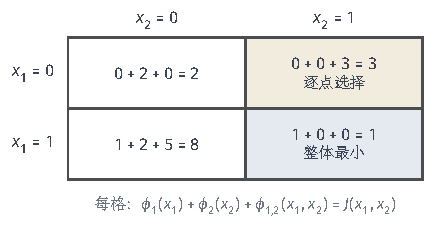
\includegraphics[width=72.383mm]{figures/01-basic-mathematics/04-graphs/tikz/c4-pairwise-config-table/figure.pdf}
  \caption{两变量成对二值函数的四种配置。行是$x_1$，列是$x_2$，每格依次写出$\phi_1(x_1)$、$\phi_2(x_2)$、$\phi_{1,2}(x_1,x_2)$与总成本$J$。逐点按一元项选择得到黄色格$(0,1)$，成本$3$；整体最小是蓝色格$(1,1)$，成本$1$。}
  \label{fig:graph-setfn-pairwise-config-table}
\end{figure}

两个变量可以枚举，$n$个变量则有$2^n$种配置。下面把四种配置的成本同时编码进一个网络的割容量，使枚举变成一次最小割计算。

\subsection{次模条件与割表示}
\label{sec:graph-setfn-cut-representation}

割容量只能累加非负的弧容量，因此能否编码取决于成对项的形状。关键条件是对每条边$\{i,j\}\in E$成立
\begin{equation}
  \phi_{i,j}(0,0)+\phi_{i,j}(1,1)\leq\phi_{i,j}(0,1)+\phi_{i,j}(1,0).
  \label{eq:graph-setfn-pairwise-submodular}
\end{equation}
它正是两元素底集$\{i,j\}$上的次模不等式：把$\phi_{i,j}$看成$\{i,j\}$上的集合函数，在式~\eqref{eq:graph-setfn-submodular-inequality}中取$X=\{i\}$、$Y=\{j\}$，左边$F(X)+F(Y)$对应$\phi_{i,j}(1,0)+\phi_{i,j}(0,1)$，右边$F(X\cup Y)+F(X\cap Y)$对应$\phi_{i,j}(1,1)+\phi_{i,j}(0,0)$。一元项是模函数，若每个成对项都满足式~\eqref{eq:graph-setfn-pairwise-submodular}，则$J$作为集合函数是次模的。上面的例子中$0+0\leq3+5$，条件成立。

\paragraph{成对项的分解}
条件~\eqref{eq:graph-setfn-pairwise-submodular}允许把一个成对项拆成常数、两个一元的线性部分和一个非负的不一致惩罚。

\begin{lemma}[成对项的分解]
\label{lem:graph-setfn-pairwise-decomposition}
设$\phi_{i,j}$满足式~\eqref{eq:graph-setfn-pairwise-submodular}，简记$p_{a,b}=\phi_{i,j}(a,b)$，令
\[
  \begin{gathered}
  w_{i,j}=\frac{p_{0,1}+p_{1,0}-p_{0,0}-p_{1,1}}{2},\\
  \alpha_i=p_{1,0}-p_{0,0}-w_{i,j},\qquad
  \alpha_j=p_{0,1}-p_{0,0}-w_{i,j}.
  \end{gathered}
\]
则$w_{i,j}\geq0$，并且对四种配置都有
\begin{equation}
  \phi_{i,j}(x_i,x_j)=p_{0,0}+\alpha_ix_i+\alpha_jx_j+w_{i,j}\,|x_i-x_j|.
  \label{eq:graph-setfn-pairwise-decomposition}
\end{equation}
\end{lemma}

\begin{proof}
$w_{i,j}\geq0$就是式~\eqref{eq:graph-setfn-pairwise-submodular}移项除以$2$。逐个代入四种配置核对右边：$(0,0)$时为$p_{0,0}$；$(1,0)$时为$p_{0,0}+\alpha_i+w_{i,j}=p_{1,0}$；$(0,1)$时为$p_{0,0}+\alpha_j+w_{i,j}=p_{0,1}$；$(1,1)$时为$p_{0,0}+\alpha_i+\alpha_j=p_{1,0}+p_{0,1}-p_{0,0}-2w_{i,j}=p_{1,1}$，最后一步代入$w_{i,j}$的定义。
\end{proof}

在例子中，$w_{1,2}=(3+5-0-0)/2=4$，$\alpha_1=5-0-4=1$，$\alpha_2=3-0-4=-1$。

\paragraph{一元项的合并与移位}
对每条边作上述分解，把常数$\phi_{i,j}(0,0)$累加起来，把线性部分$\alpha_ix_i$、$\alpha_jx_j$并入相应元素的一元项。记合并后的一元项为$\psi_i$，即$\psi_i(0)=\phi_i(0)$，$\psi_i(1)=\phi_i(1)$加上与$i$关联的各边分解出的$\alpha_i$。$\psi_i$可能取负值，而容量必须非负，所以再令$m_i=\min\{\psi_i(0),\psi_i(1)\}$，$\tilde\psi_i=\psi_i-m_i$，两种状态的成本都减去同一个数，$\tilde\psi_i$的两个值非负且至少一个为零。移出的数另行累计成常数
\[
  K=\sum_{\{i,j\}\in E}\phi_{i,j}(0,0)+\sum_{i\in V}m_i .
\]
于是对每个配置都有
\begin{equation}
  J(\bm x)=K+\sum_{i\in V}\tilde\psi_i(x_i)+\sum_{\{i,j\}\in E}w_{i,j}\,|x_i-x_j|,
  \label{eq:graph-setfn-shifted-objective}
\end{equation}
右边除常数$K$外各项都非负。在例子中，$\psi_1=(0,\,1+1)=(0,2)$，$\psi_2=(2,\,0-1)=(2,-1)$；$m_1=0$，$m_2=-1$，所以$\tilde\psi_1=(0,2)$，$\tilde\psi_2=(3,0)$，$K=0+0+(-1)=-1$。

\paragraph{网络构造}
由式~\eqref{eq:graph-setfn-shifted-objective}构造有向网络：顶点为$V\cup\{s,t\}$；对每个$i\in V$，建弧$s\to i$，容量$\tilde\psi_i(1)$，以及弧$i\to t$，容量$\tilde\psi_i(0)$；对每条边$\{i,j\}\in E$，建方向相反的两条弧$i\to j$与$j\to i$，容量都是$w_{i,j}$。容量为零的弧可以省略。规定源侧的元素取$0$、汇侧的元素取$1$，即配置$\bm x$对应$s$--$t$割$(S_{\bm x},\bar S_{\bm x})$，其中$S_{\bm x}=\{s\}\cup\{i:x_i=0\}$。用最小割求解这类问题的方法常称为\term{图割}（graph cut）。

\begin{theorem}[成对二值函数的割表示]
\label{thm:graph-setfn-cut-representation}
设式~\eqref{eq:graph-setfn-pairwise-objective}中的成本都是有限实数，且每个成对项满足式~\eqref{eq:graph-setfn-pairwise-submodular}。则在上面构造的网络中，配置与$s$--$t$割一一对应，并且每个配置$\bm x$对应的割容量等于$J(\bm x)-K$。因此最小割对应的配置是$J$的最小点。
\end{theorem}

\begin{proof}
任一$s$--$t$割的源侧都含$s$、不含$t$，由$V$中哪些元素在源侧唯一确定，所以割与配置一一对应。割容量只累计从源侧指向汇侧的弧，逐类计算。若$x_i=0$，$i$在源侧，弧$i\to t$跨出，计入$\tilde\psi_i(0)$，弧$s\to i$两端都在源侧，不计入；若$x_i=1$，$i$在汇侧，弧$s\to i$跨出，计入$\tilde\psi_i(1)$，弧$i\to t$两端都在汇侧，不计入。两种情形合起来恰好计入$\tilde\psi_i(x_i)$。对边$\{i,j\}$，若$x_i=x_j$，两条弧都不跨越；若$x_i\neq x_j$，两条反向弧中恰有一条从源侧指向汇侧，计入一次$w_{i,j}$。合起来恰好计入$w_{i,j}|x_i-x_j|$。所以割容量等于式~\eqref{eq:graph-setfn-shifted-objective}右边去掉$K$，即$J(\bm x)-K$。$K$与配置无关，最小化割容量与最小化$J$是同一件事。
\end{proof}

在例子中，网络有弧$s\to1$（容量$2$）、$2\to t$（容量$3$）、$1\to2$与$2\to1$（容量都是$4$），弧$1\to t$与$s\to2$容量为零。表~\ref{tab:graph-setfn-cut-check}逐个核对四种配置：割容量都比$J$大$1$，即$-K$。

\begin{table}[!htb]
  \centering
  \begin{tabular}{cccc}
    \toprule
    配置$\bm x$ & 源侧 & 跨出的正容量弧 & 割容量 / $J(\bm x)$ \\
    \midrule
    $(0,0)$ & $\{s,1,2\}$ & $2\to t$ & $3$ / $2$ \\
    $(0,1)$ & $\{s,1\}$ & $1\to2$ & $4$ / $3$ \\
    $(1,0)$ & $\{s,2\}$ & $s\to1$，$2\to t$，$2\to1$ & $9$ / $8$ \\
    $(1,1)$ & $\{s\}$ & $s\to1$ & $2$ / $1$ \\
    \bottomrule
  \end{tabular}
  \caption{两变量例子中四种配置的割容量与原目标值。源侧元素取$0$、汇侧元素取$1$；每行割容量都等于$J(\bm x)+1$，相差的常数是$-K=1$，所以割容量最小的$(1,1)$也是$J$的最小点。}
  \label{tab:graph-setfn-cut-check}
\end{table}

\paragraph{条件不成立时}
若某个成对项违反式~\eqref{eq:graph-setfn-pairwise-submodular}，引理给出的$w_{i,j}$为负，网络中就会出现负容量的弧。第~\ref{sec:graph-max-flow}节的流值与割容量的关系建立在非负容量之上，负容量时不能直接使用。例如奖励两个变量取值不同的成对项$\phi_{i,j}(0,1)=\phi_{i,j}(1,0)=0$、$\phi_{i,j}(0,0)=\phi_{i,j}(1,1)=1$就违反条件，这时的最小化一般不能化为一次最小割。

\subsection{最小割求解与解的恢复}
\label{sec:graph-setfn-cut-solving}

\paragraph{求解步骤}
构造网络后，用第~\ref{sec:graph-max-flow}节的Edmonds--Karp算法求最大流。算法停止时，残量网络中从$s$可达的顶点集合是一个最小割的源侧；把其中的元素标为$0$，其余元素标为$1$，就得到最优配置$\hat{\bm x}$。结果可以独立核对：直接按式~\eqref{eq:graph-setfn-pairwise-objective}计算$J(\hat{\bm x})$，它应等于最大流值加$K$。由于最大流值等于最小割容量，这个等式同时证明了$\hat{\bm x}$的最优性，而不必相信算法实现本身。

\paragraph{两变量例子的求解}
网络中从$s$到$t$只有一条正容量路径$s\to1\to2\to t$，瓶颈为$\min\{2,4,3\}=2$。沿它增广$2$个单位后，$s\to1$的正向残量为零，$s\to2$本来容量为零，所以残量网络中从$s$出发哪里也到不了，可达集合是$\{s\}$。最小割容量$2$等于流值，两个元素都在汇侧，得到$\hat{\bm x}=(1,1)$。代回原目标，$J(1,1)=1+0+0=1=2+K$，与图~\ref{fig:graph-setfn-pairwise-config-table}中的枚举结果一致。图~\ref{fig:graph-setfn-st-cut-construction}把这个最小割与配置$(0,1)$对应的割并排比较。

\begin{figure}[!htb]
  \centering
  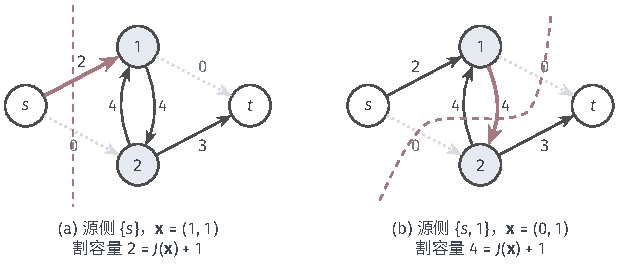
\includegraphics[width=104.687mm]{figures/01-basic-mathematics/04-graphs/tikz/c4-st-cut-construction/figure.pdf}
  \caption{两变量例子的$s$--$t$网络。弧旁数字是容量，灰色点线是容量为零的弧；红色虚线分开源侧与汇侧，红色粗弧是跨出割的正容量弧。源侧元素取$0$、汇侧元素取$1$。(a) 最小割，源侧$\{s\}$，只割断$s\to1$，容量$2$，对应$(1,1)$；(b) 源侧$\{s,1\}$，割断$1\to2$，容量$4$，对应逐点选择得到的$(0,1)$。两种情况的割容量都等于$J(\bm x)+1$。}
  \label{fig:graph-setfn-st-cut-construction}
\end{figure}

\paragraph{开销}
网络有$n+2$个顶点，弧数$a\leq2n+2m$，其中$m=|E|$；计算分解、合并一元项和建弧都只需扫描一遍元素与边，用时$O(n+m)$。主要开销在最大流：按第~\ref{sec:graph-max-flow}节的分析，Edmonds--Karp算法需要$O(na^2)$次算术与比较操作，代入$a=O(n+m)$即$O(n(n+m)^2)$。与枚举$2^n$种配置相比，这是多项式规模的计算。

\paragraph{与前两节的比较}
本节与前两节都在子集上做选择，但条件和结论不同。前两节在基数或预算约束下最大化单调次模函数，得到的是近似解，保证依赖单调性、次模性和约束的形式。本节最小化可以写成一元项加满足式~\eqref{eq:graph-setfn-pairwise-submodular}的成对项的函数，没有额外约束，得到的是精确解，依据是割表示。在本节的问题上再加“恰好选$k$个”这样的数量限制，割与配置的对应就不再保持约束；含三个及以上变量的高阶项、违反条件的成对项，以及每个变量有三种以上取值的问题，也都不能直接套用这个构造。一般次模函数的最小化另有专门的算法，超出本书范围。
